\begin{frame}{Semidefinite program}
%  \begin{columns}
    %\begin{column}{0.48\textwidth}
      \begin{equation*}
        \label{eq:sdp_standard}
        \begin{array}{rl}
          \min\limits_{Q \in \SymK[N]} & \la C, Q \ra\\
          \text{subject to:} & \la A_i, Q \ra = b_i, \quad i=1,2,\ldots,m\\
          & Q \succeq 0.
        \end{array}
      \end{equation*}
      \pause
    %\end{column}
    %\begin{column}{0.48\textwidth}
      Is $p(x) = x^6 - 2x^4 + 2x^2$ always non-negative? $\to$ sum of squares relaxation: Does there exist psd matrix $Q$ s.t. 
      \[p(x) = X^\Tr Q X = \langle X X^\Tr, Q \rangle ?\]
      
      \comment{
      Feasibility problem with
      $$
      X =
      \begin{bmatrix}
        x^3\\
        x^2\\
        x
      \end{bmatrix},
      XX^\Tr =
      \begin{bmatrix}
        x^6 & x^5 & x^4\\
        \cdot & x^4 & x^3\\
        \cdot & \cdot & x^2
      \end{bmatrix},
      A_{x^6} =
      \begin{bmatrix}
        1 & 0 & 0\\
        \cdot & 0 & 0\\
        \cdot & \cdot & 0
      \end{bmatrix},
      A_{x^5} =
      \begin{bmatrix}
        0 & 1 & 0\\
        \cdot & 0 & 0\\
        \cdot & \cdot & 0
      \end{bmatrix},\; \text{etc.}
      $$
      $b = (b_i)$ is the vector of coefficients of $p$. }
%       $$
%       A_{x^4} =
%       \begin{bmatrix}
%         0 & 0 & 1\\
%         \cdot & 1 & 0\\
%         \cdot & \cdot & 0
%       \end{bmatrix},
%       A_{x^3} =
%       \begin{bmatrix}
%         0 & 0 & 0\\
%         \cdot & 0 & 1\\
%         \cdot & \cdot & 0
%       \end{bmatrix},
%       A_{x^2} =
%       \begin{bmatrix}
%         0 & 0 & 0\\
%         \cdot & 0 & 0\\
%         \cdot & \cdot & 1
%       \end{bmatrix}.
%       $$
    %\end{column}
%  \end{columns}

      %\noindent {\tiny Gatermann, Parrilo, \emph{{S}ymmetry groups, semidefinite programs, and sums of squares}, Journal of Pure and Applied Algebra, 2004: Example~5.1}
\end{frame}

\begin{frame}{Problems}
  For $n$-variate polynomial of degree $2d$:
  \[N = {n + d \choose n},\qquad m = {n + 2d \choose n}.\]
  \pause
  \vspace*{-0.3in}
  \begin{itemize}
    \item interior point solvers ($\bigoh(mN^{3.5} + m^2N^{2.5})$)\\\comment{CSDP, DSDP, Hypatia, MOSEK, SDPA, ...}
    \item Alternating Direction Method of Multipliers\\
    \comment{CDCS, COSMO, SCS, ...}
    \item Low rank approximation of $Q$, (Scaled) dominantly diagonal matrices, Newton conjugate gradient, Primal-dual hybrid gradient...
  \end{itemize}

\end{frame}


\begin{frame}{Simplifying the original program}

\begin{itemize}
%  \item Linear projection based \\\comment{(find a low rank linear subspace for $\SymK[N]$ where solutions live)}
  \item Block-diagonalization \\\comment{(represent $Q$ as block diagonal direct sum of psd matrices)}
  \begin{enumerate}
    \item Chordal decomposition \comment{(exploit sparsity pattern in $A_i$s)}
    \item Wedderburn(-Artin) decomposition for matrix algebras \\\comment{(group symmetry, general *-algebras, Jordan algebras, ...)}
  \end{enumerate}
\end{itemize}
\pause

\vspace*{0.3in}
\footnote[]{\tiny
Disclaimer: This is not new, has been re-invented several times in the literature. See e.g. \gatpar
}


\end{frame}

\begin{frame}{Group symmetry invariance: Example}
\vspace*{0.2in}
  \begin{block}{Robinson form}
      $$
      R(x,y) = x^6 + y^6 - x^4y^2 - y^4x^2 - x^4 - y^4  + 3x^2y^2 - x^2 - y^2 + 1.
      $$
  \vspace{-.1in}
      $R$ is invariant under the following operations \textbf{on monomials}
      \begin{align*}
        \alpha_1 \colon (x, y) & \mapsto (y, x)\\
        \alpha_2 \colon (x, y) & \mapsto (-y, x)
      \end{align*}
    \\[-0.6in]
    
    \comment{$\{ \alpha_1, \alpha_2 \}$ generate a set of $8$ symmetries -- the dihedral group $D_4$.}
  \end{block}
    \pause

  \begin{itemize}
    \item symmetry of monomials $\longrightarrow$ symmetry of constraints
    \item symmetry of monomials $\longrightarrow$ symmetry of psd matrix $Q$
    \item invariant problem = problem "remains the same" under those symmetries
  \end{itemize}

\end{frame}


\begin{frame}[standout]{Misleading quote of the day}
  
  \begin{quote}
    \noindent The \textbf{structure} of simplifications that can be derived from a symmetry pattern does \textbf{not} depend on the optimization problem.
  \end{quote}
  
\end{frame}

\begin{frame}{Block decomposition from symmetries}
  Any matrix $Q$ invariant under group symmetries\\
  admits a block-diagonal structure.

\begin{center}
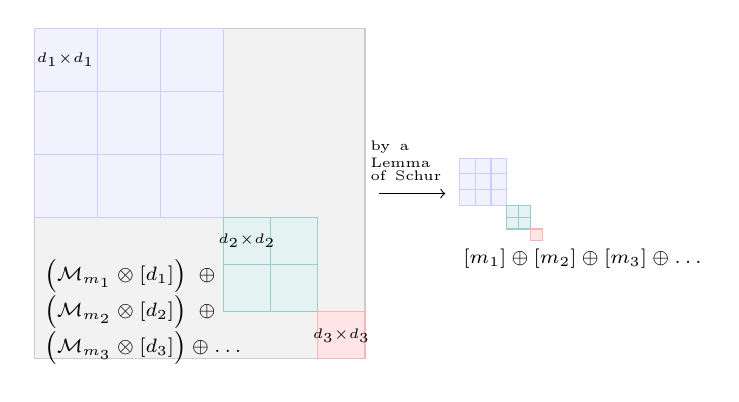
\begin{tikzpicture}[scale=0.6]
\draw [thin, draw=black!20, fill=black!5] (0,0) (7,7) rectangle (0,0);
\pause
\draw [thin, draw=blue!20, fill=blue!5] (0,7) rectangle (4,3);
\draw [thin, draw=teal!40, fill=teal!10] (4,3) rectangle (6,1);
\draw [thin, draw=red!30, fill=red!10] (6,1) rectangle (7,0);
\node () at (0,0.5) [anchor=west] {\scriptsize{$\SymK[N_1] \oplus \SymK[N_2] \oplus \SymK[N_3] \oplus \ldots$}};

\pause
\begin{scope}[shift={(0,0)}]
\draw [thin, draw=black!20, fill=black!5] (0,0) rectangle (7,7);
\begin{scope}[shift={(0,3)}, scale=1.333]
  \draw [thin, draw=blue!20, fill=blue!5] (0,0) grid (3,3) rectangle (0,0);
\end{scope}
\draw [thin, draw=teal!40, fill=teal!10] (6,1) grid (4,3) rectangle (6,1);
\draw [thin, draw=red!30, fill=red!10] (7,0) grid (6,1) rectangle (7,0);
\node () at (0,1) [anchor=west, text width=4cm] {\scriptsize{$\left(\mathcal{M}_{m_1}\otimes\SymK[d_1]\right) \oplus \left(\mathcal{M}_{m_2}\otimes\SymK[d_2]\right) \oplus \left(\mathcal{M}_{m_3}\otimes\SymK[d_3]\right) \oplus \ldots$}};

\begin{scope}[shift={(0,7)}]
  \node () at (.66,-.66) [anchor=center] {\tiny{$d_1 \hspace{-0.75ex} \times \hspace{-0.75ex} d_1$}};
\end{scope}

\begin{scope}[shift={(4,3)}]
  \node () at (.5,-.5) [anchor=center] {\tiny{$d_2 \hspace{-0.75ex} \times \hspace{-0.75ex} d_2$}};
\end{scope}

\begin{scope}[shift={(6,1)}]
  \node () at (.5,-.5) [anchor=center] {\tiny{$d_3 \hspace{-0.75ex} \times \hspace{-0.75ex} d_3$}};
\end{scope}


\end{scope}

\pause


\draw [->] (7.3, 3.5) -- (8.7, 3.5);
\node () at (8.2, 4.2) [anchor=center, text width=1.3cm] {\tiny by a Lemma\\[-0.1in] of Schur};

\begin{scope}[shift={(9,2.5)}, scale=0.25]
% \draw [thin, draw=black!20, fill=black!5] (0,0) rectangle (7,7);
\begin{scope}[shift={(0,3)}, scale=1.333]
  \draw [thin, draw=blue!20, fill=blue!5] (0,0) grid (3,3) rectangle (0,0);
\end{scope}
% \draw [thin, draw=blue!20, fill=blue!5] (4,3) grid (0,7) rectangle (4,3);
\draw [thin, draw=teal!40, fill=teal!10] (6,1) grid (4,3) rectangle (6,1);
\draw [thin, draw=red!30, fill=red!10] (7,0) grid (6,1) rectangle (7,0);
\node () at (-0.5,-1.5) [anchor=west] {\scriptsize{$\SymK[m_1] \oplus \SymK[m_2] \oplus \SymK[m_3] \oplus \ldots$}};
\end{scope}

% \draw [thin, draw=black!20, fill=black!5] (0,0) grid (7,7) rectangle (0,0);

\end{tikzpicture}
\end{center}

\uncover<5->{\comment{Those isomorphims and minimal rank projections live in the group *-algebra in a basis-free form!}}

\end{frame}

\begin{frame}[fragile]{Example: {\texttt{SymbolicWedderburn.jl}}}
\scriptsize
\begin{minted}{julia}
  using PermutationGroups, DynamicPolynomials
  using SymbolicWedderburn
  G = PermGroup([perm"(1,2)", perm"(1,2,3,4)"]) # Sym(4)
  @polyvar x[1:4];  basis = monomials(x, 0:2) # 15 monomials
  symmetry_adapted_basis(Rational{Int}, G, VariablePermutation(), basis, 
      semisimple=true)
\end{minted}
\normalsize
\textbf{Isotypical}/\textbf{semisimple} blocks when acting on \mintinline{julia}|basis|:
\tiny
\[
  B_1 = \begin{bmatrix}
          1\\
          x_1 + x_2 + x_3 + x_4\\
          x_{1}x_{2} + x_{1}x_{3} + x_{1}x_{4} + x_{2}x_{3} + x_{2}x_{4} + x_{3}x_{4}\\
          x_{1}^{2} + x_{2}^{2} + x_{3}^{2} + x_{4}^{2}
        \end{bmatrix}
  \qquad
  B_2 = \begin{bmatrix}
        x_{1} - x_{4}\\
        x_{2} - x_{4}\\
        x_{3} - x_{4}\\
        x_{2}^{2} - x_{4}^{2}\\
        x_{3}^{2} - x_{4}^{2}\\
        x_{1}^{2} - x_{4}^{2}\\
        x_{1}x_{2} - x_{3}x_{4}\\
        x_{1}x_{3} - x_{2}x_{4}\\
        x_{1}x_{4} - x_{2}x_{3}\\
        \end{bmatrix}
  \qquad
  B_3 = \begin{bmatrix}
        x_{1}x_{2} - x_{1}x_{4} - x_{2}x_{3} + x_{3}x_{4}\\
        x_{1}x_{3} - x_{1}x_{4} - x_{2}x_{3} + x_{2}x_{4}
        \end{bmatrix}
\]

\comment{We went from $15\times 15$-psd constrain to sizes $(4\times 4, 9\times 9, 2\times 2)$.}
  %\[V \cong (V_1' \oplus V_1') \oplus V_2' \oplus V_3', \qquad m_1 = 2, \quad m_2 = m_3 = 1.\]
\end{frame}

\begin{frame}[fragile]{Example: {\texttt{SymbolicWedderburn.jl}}}
\vspace*{0.2in}
\scriptsize

\begin{minted}{julia}
  # [ ... ]
  symmetry_adapted_basis(Rational{Int}, G, VariablePermutation(), basis
    [, semisimple=false])
\end{minted}
\normalsize
\textbf{Simple} blocks when acting on \mintinline{julia}|basis|:
\tiny
\[
  B_1 = \begin{bmatrix}
          1\\
          x_1 + x_2 + x_3 + x_4\\
          x_{1}x_{2} + x_{1}x_{3} + x_{1}x_{4} + x_{2}x_{3} + x_{2}x_{4} + x_{3}x_{4}\\
          x_{1}^{2} + x_{2}^{2} + x_{3}^{2} + x_{4}^{2}
        \end{bmatrix}
  \qquad
  B_2 = \begin{bmatrix}
        \frac{1}{3}(3x_{1} - x_{2} - x_{3} - x_{4})\\
        \frac{1}{3}(3x_{1}^{2} - x_{2}^{2} - x_{3}^{2} - x_{4}^{2})\\
        x_{1}x_{2} + x_{1}x_{3} + x_{1}x_{4} - x_{2}x_{3} - x_{2}x_{4} - x_{3}x_{4}
        \end{bmatrix}
\]
\[
  B_3 = \begin{bmatrix}
        \frac{1}{2}(2x_{1}x_{2} - x_{1}x_{3} - x_{1}x_{4} - x_{2}x_{3} - x_{2}x_{4} + 2x_{3}x_{4})
        \end{bmatrix}
\]

\comment{We went from $(4\times 4, 9\times 9, 2\times 2)$-psd constraints to sizes $(4\times 4, 3\times 3, 1\times 1)$.}\\[0.1in]

\end{frame}

\begin{frame}{Large scale example}

  \begin{itemize}
    \item Optimization problem from geometric group theory\footnote{Kaluba, M., Nowak, P.W. \& Ozawa, N. $\operatorname{Aut}(F_5)$ has property (T). \textit{Math. Ann}. \textbf{375}, 1169–1191 (2019). \url{https://doi.org/10.1007/s00208-019-01874-9}}
    \item psd-constraint of size $4\,641\times 4\,641$, $~1.1\cdot 10^7$ constraints
    \item symmetry group: $S_2 \wr S_5$ ($3840$ elements)
    \item After symmetrization:
      \begin{itemize}
        \item $29$-blocks (largest: $58\times 58$), $13\,232$ variables in total
        \item $7\,230$ constraints
      \end{itemize}
    \item Solvable in 20 minutes to $\varepsilon \sim 10^{-12} $!
  \end{itemize}

\end{frame}

\begin{frame}
\begin{center}
\vfill
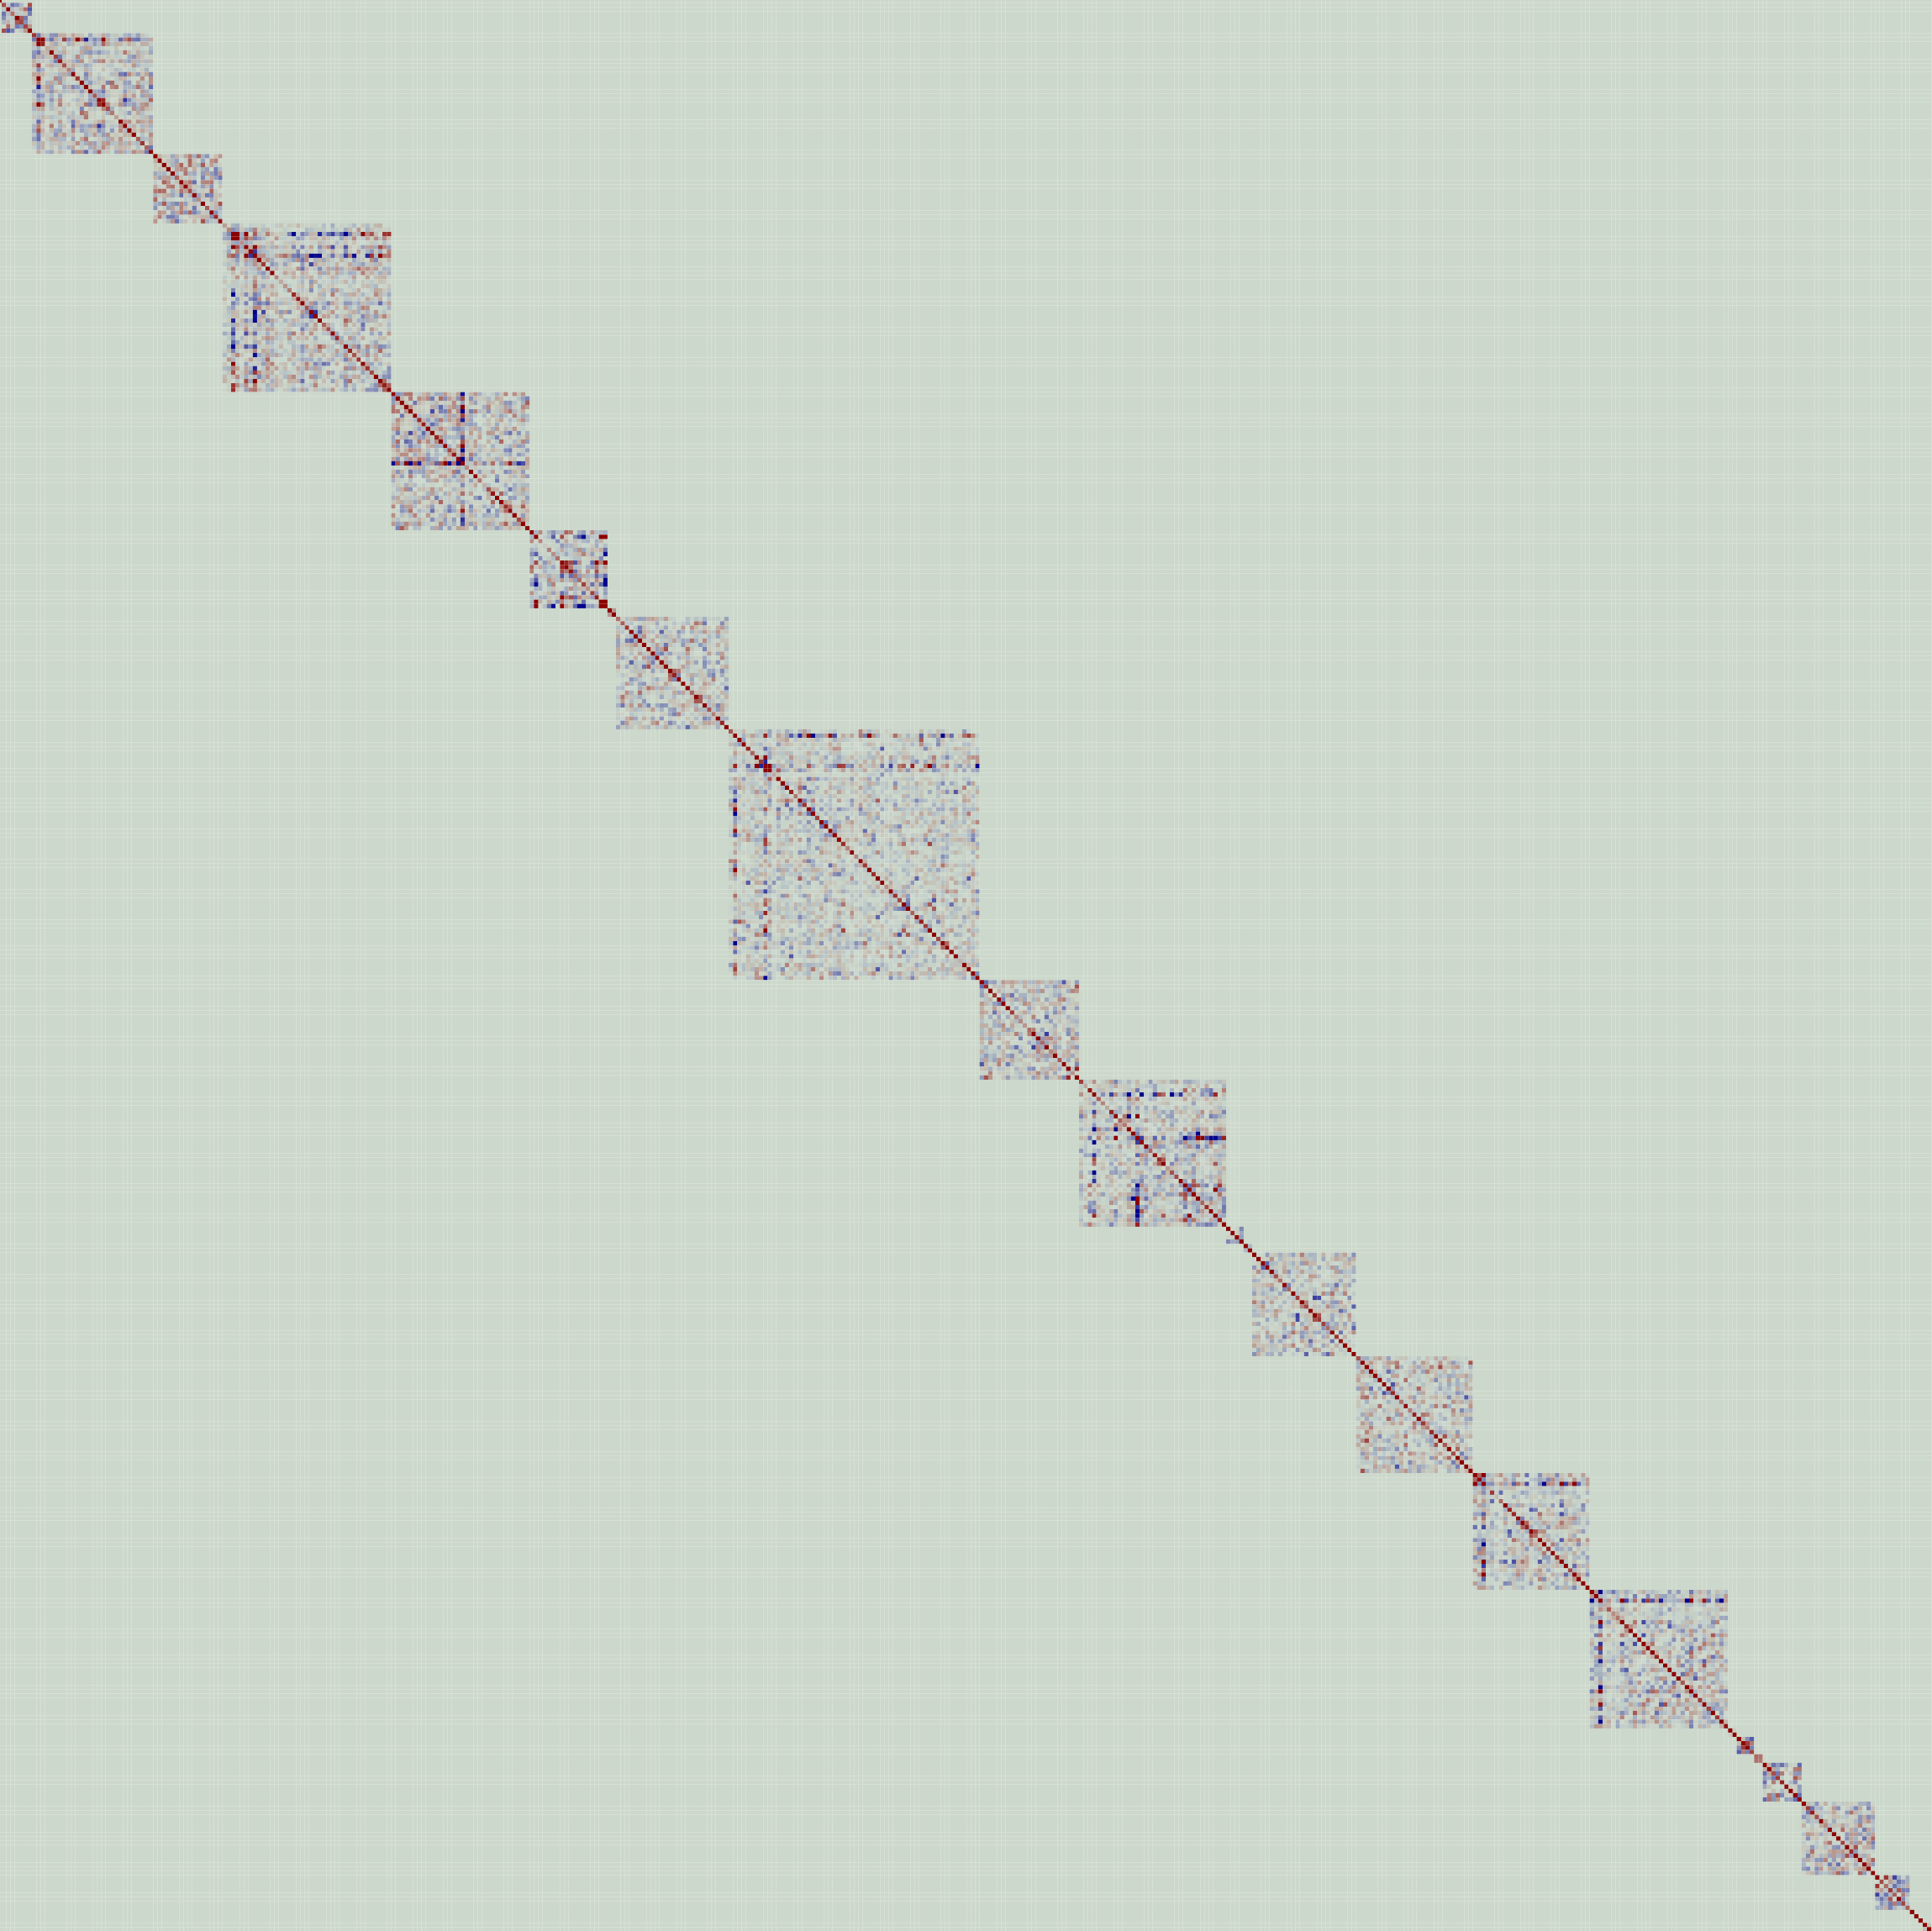
\includegraphics[height=\textheight]{AutF5_blocks.png}
\vfill
\end{center}
\end{frame}

\begin{frame}
\centering
\begin{tikzpicture}[scale=0.9]
\draw [thin, draw=black!20, fill=blue!5] (0,0) grid (10.18,-10.18) rectangle (0,0);
\node at (6.5, -9.5) {Original psd constraint ($4\, 641 \times 4\, 641$)};
\node (ssdp) at (.5,-.5) {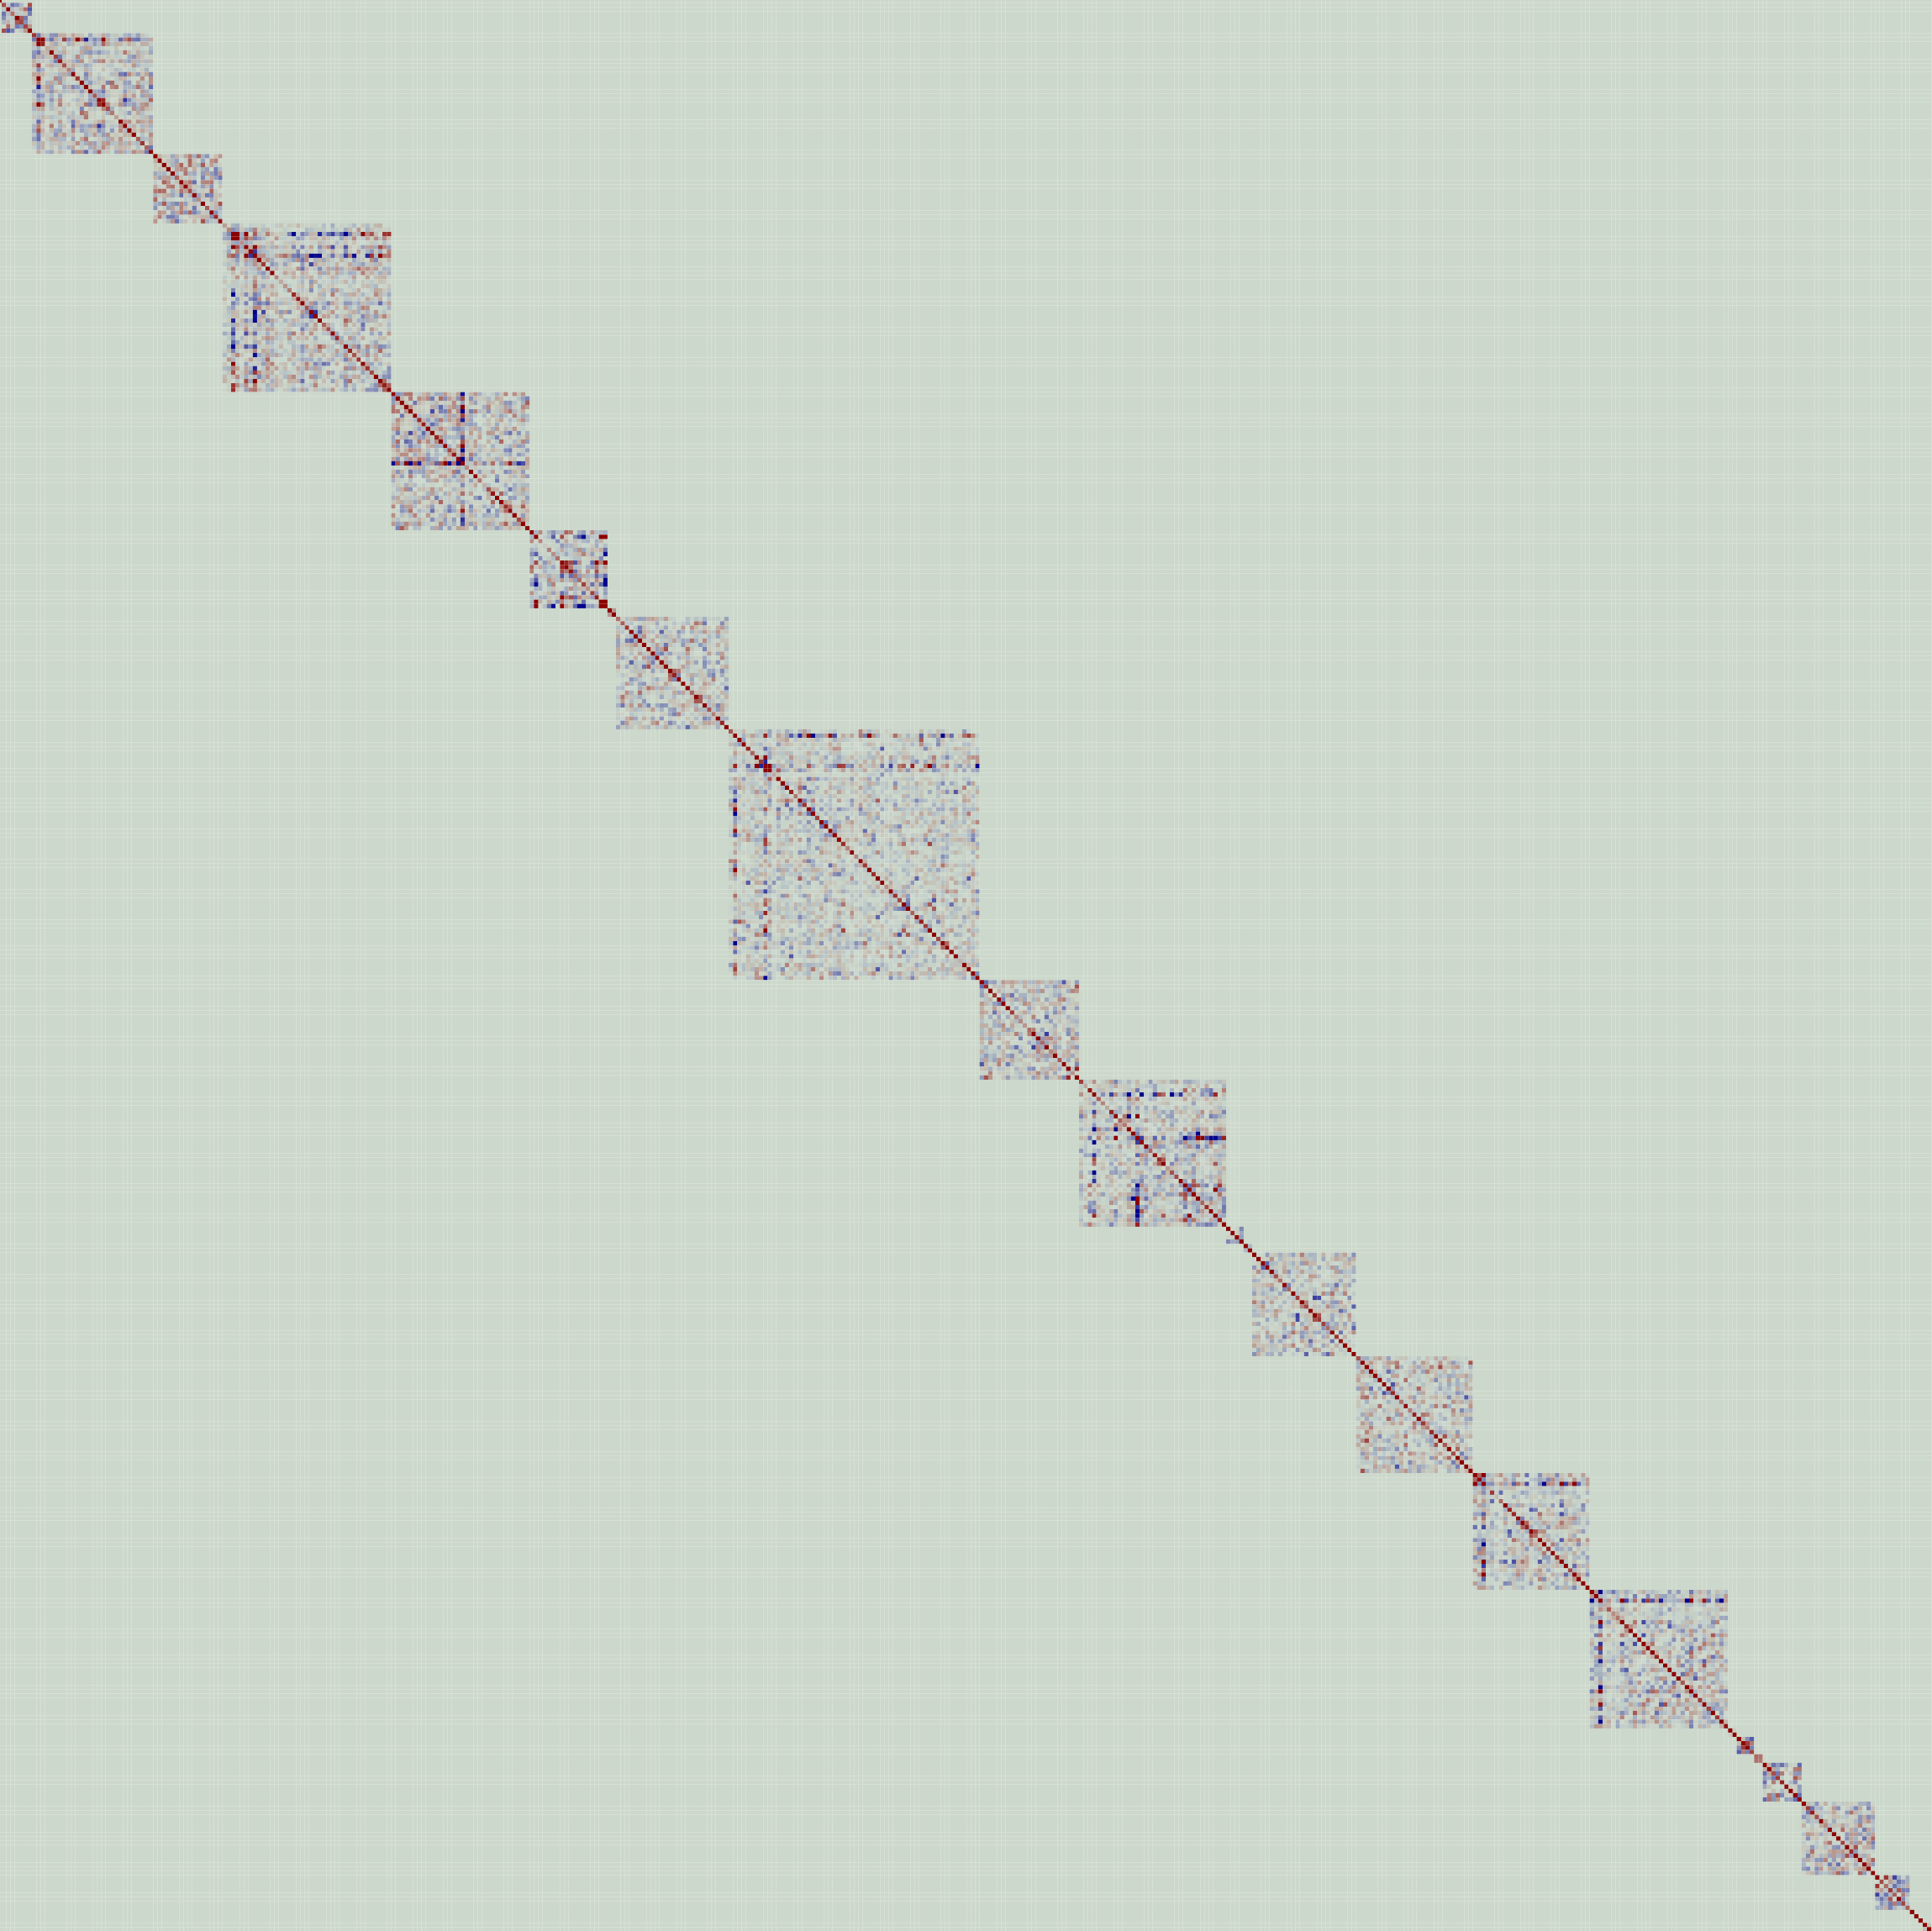
\includegraphics[width=0.9cm]{AutF5_blocks.png}};
\node (label) at (4.5,-.5) {diagonalized psd ($\subset 448\times 448$)};
\draw [->] (label.west) -- (ssdp.east);
\end{tikzpicture}


\end{frame}



\begin{frame}[fragile]
\scriptsize
\begin{minted}{julia}
C = ... # objective
A = ... # constraint matrices
b = ... # constraint values
basis_cnstr = ... # basis in which b is written and G acts on
basis_psd = ... # basis for the psd constraint Q

G = ... # a group, <: instance of GroupsCore.Group
action = ... # instance of SymbolicWedderburn.Action
wedderburn = WedderburnDecomposition(Float64, G, action, basis_cnstr, basis_psd)

m = JuMP.Model()
psds = [ JuMP.@variable(m, [1:d, 1:d] in PSDCone())
    for d in size.(direct_summands(wedderburn), 1)]

for iv in invariant_vectors(wedderburn)
    biv = dot(b, iv)
    Ai_iv = invariant_constraint(A, iv) # ~ weighted average
    Aπs = SymbolicWedderburn.diagonalize(Ai_iv, wedderburn)
    JuMP.@constraint m sum(
        dot(Aπ, Pπ) for (Aπ, Pπ) in zip(Aπs, psds) if !iszero(Aπ)
    ) == biv
end
JuMP.@objective(m, Max, sum(dot(C, iv) for iv in invariant_vectors(wedderburn)))

\end{minted}

\end{frame}


\begin{frame}{Behind the scenes: \texttt{SymbolicWedderburn.jl}}
    \begin{itemize}
      \item given action e.g. on monomials, \alert{induce} the action to the whole basis
      \item compute \alert{character table} of the group $\longrightarrow$ central projections
      \item for each central projection find minimal rank projection (symbolically, in the group *-algebra)
      \item evaluate the projections in the action on the basis $\longrightarrow$ \alert{matrix projections}
    \end{itemize}
\end{frame}


\begin{frame}{Exploiting the symmetry: reducing constraints}

  Instead of using all $\langle A_i, Q \rangle = b_i$ it's enough to use
    \[\left\langle \frac{1}{|G|}\sum_g g(A_i), Q \right\rangle = b_{[i]},\]
    for each ``invariant set'' of the original constraints.
    \\[0.2in]\comment{In the example: instead of looking at $b_x$ (the coefficient at $x$), or $b_y$ separately, we should be looking at $b_{\frac{x+y}{2}} = \left\langle\frac{1}{2}(A_x + A_y), Q \right\rangle$}
    \\[0.2in]\comment{This corresponds to finding a basis for the ``invariants ring'' $\R[x]^G$.}

\end{frame}




